\documentclass{article}

\usepackage{arxiv}

\usepackage[utf8]{inputenc}
\usepackage[T1]{fontenc}
\usepackage[strings]{underscore}
\usepackage{hyperref}
\usepackage{url}
\usepackage{booktabs}
\usepackage{amsfonts}
\usepackage{amsmath}
\usepackage{amssymb}
\usepackage{nicefrac}
\usepackage{microtype}
\usepackage{cleveref}
\usepackage{graphicx}
\usepackage{natbib}
\usepackage{listings}
\usepackage{xcolor}
\usepackage{seqsplit}
\usepackage{tikz}
\usepackage{multirow}
\usepackage{framed}
\usepackage{needspace}
\usepackage{placeins}
\usetikzlibrary{positioning,arrows.meta,fit,backgrounds,shapes.multipart,shapes.geometric,calc}

\newcounter{algo}
\crefname{algo}{Algorithm}{Algorithms}
\Crefname{algo}{Algorithm}{Algorithms}
\newenvironment{algobox}[1]{%
  \begin{framed}\refstepcounter{algo}\textbf{\sffamily\small Algorithm \thealgo: #1}\vspace{3pt}\hrule\vspace{5pt}
  \small\ttfamily\raggedright
}{%
  \end{framed}
}

\lstset{
  basicstyle=\ttfamily\footnotesize,
  breaklines=true,
  columns=fullflexible,
  frame=single,
  framerule=0.4pt,
  backgroundcolor=\color{white},
  showstringspaces=false
}

\title{Kernel Borderlands: An eBPF-Based Behavioral Detection and
Multi-Agent Containment Architecture for Linux Server Workloads}

\author{
  Pardhu Sri Rushi Varma Konduru \\
  Dept.\ of Cybersecurity, ECE \& IoT \\
  Malla Reddy University, Hyderabad \\
  \texttt{2311CS040089@mallareddyuniversity.ac.in}
  \And
  Tejaswini Kandukoori \\
  Dept.\ of Cybersecurity, ECE \& IoT \\
  Malla Reddy University, Hyderabad \\
  \texttt{2311CS040077@mallareddyuniversity.ac.in}
  \And
  Karthik Kanne \\
  Dept.\ of Cybersecurity, ECE \& IoT \\
  Malla Reddy University, Hyderabad \\
  \texttt{2311CS040080@mallareddyuniversity.ac.in}
  \And
  Rupa Yeshvitha Karedla \\
  Dept.\ of Cybersecurity, ECE \& IoT \\
  Malla Reddy University, Hyderabad \\
  \texttt{2311CS040082@mallareddyuniversity.ac.in}
}

\renewcommand{\shorttitle}{Kernel Borderlands}
\renewcommand{\headeright}{}
\renewcommand{\undertitle}{}
\date{}

\hypersetup{
pdftitle={Kernel Borderlands: An eBPF-Based Behavioral Detection and Multi-Agent Containment Architecture for Linux Server Workloads},
pdfauthor={Kernel Borderlands Team},
}

\begin{document}
\maketitle

\begin{abstract}
Kernel Borderlands (KB) is a kernel-level runtime defense framework for
Linux composed of five implemented subsystems --- an eBPF-based Ring-0
sensor (\texttt{kb-core}), a Go control plane for scoring, storage, and
enforcement (\texttt{kb-control-plane}), a Python multi-agent swarm for
adaptive response (\texttt{kb-aads}), a stateless Rust integrity
watchdog (\texttt{kb-checker}), and a set of operator interfaces
(\texttt{kb-op}) --- plus a briefly-noted extended hardware feature
developed in parallel by a dedicated sub-team in a separate repository,
the Node Out-of-Band Module for Attestation \& Defense (NOMAD),
intended to eventually move the system's last line of defense off the
monitored host entirely. This paper documents the design,
implementation history, and current status of every subsystem,
including defects found and fixed along the way and defects still
open, and gives a unified mathematical formulation of the framework's
learned and rule-based decision procedures: the Containment and Jury
reinforcement-learning policies, Judge/Jury/Executor quorum consensus,
the courthouse severity ladder for supervising the agent swarm itself,
and the Shannon-entropy/CUSUM statistics underlying beaconing and
slow-exfiltration detection. Relative to the project's earlier state,
this revision reports newly trained and live-verified components (a
Jury consensus policy reaching 100.0\% held-out test accuracy and 0\%
false-negative rate on 908 samples), newly implemented swarm roles
(rule-based Patroller and Healer agents, a mechanically-sequenced
Containment militia, dedicated signal-relay actors, and a
\texttt{SwarmRegistry}-backed courthouse oversight mechanism for the
agent swarm itself), a signed critical-workload policy format using
Ed25519, and a severity-escalation and exfiltration-detection pipeline
on the control plane. A source-level security audit conducted across
four of the five implemented subsystems re-verified every previously
reported open defect directly against current source rather than
carrying old claims forward; the great majority --- an unauthenticated
HTTP API, a telemetry-reset containment bug, an LSM fail-open ordering
issue, three JJE consensus defects, and more --- turned out to already
be fixed in team history that simply predated when this audit's text
was first drafted, and one genuinely open defect (an audit-chain
integrity check silently masking a class of I/O error) is fixed in this
revision with a dedicated regression test. Where a subsystem or feature
is incomplete, stubbed, or under active parallel development elsewhere
(NOMAD) at the time of writing, we say so explicitly rather
than omitting it or implying a maturity the code or the design review
does not support.
\end{abstract}

\twocolumn

\keywords{eBPF \and Linux security \and runtime containment \and
multi-agent systems \and reinforcement learning \and intrusion
detection \and distributed systems \and hardware root of trust \and
trusted platform module}

\begin{center}
\small \textbf{Code availability.} The full source referenced
throughout this paper is available at
\url{https://github.com/pardhuvarmax/kernel-borderlands} \citep{kbrepo}.
\end{center}

\section{Introduction}
\label{sec:intro}

Runtime defense for Linux hosts increasingly relies on kernel-level
observability: extended Berkeley Packet Filter (eBPF) programs attached
to LSM hooks, tracepoints, and kprobes observe process behavior at
Ring 0 with low overhead \citep{gregg2019bpf}, building
on packet-filtering foundations dating back to the original BSD Packet
Filter. Observability alone is
not response --- a runtime defense system must also decide, act, and be
able to prove that its own decision trail has not been tampered with
after the fact, and, if the goal is to defend against a full kernel
compromise rather than merely detect one, it must eventually confront
the fact that a Ring-0 attacker shares every software component's trust
domain, watchdogs included. Kernel Borderlands (KB) \citep{kbrepo} is
organized around an observe-score-decide-enforce-audit loop, implemented
across five cooperating, independently substantial subsystems ---
\texttt{kb-core} (\S\ref{sec:core}), \texttt{kb-control-plane}
(\S\ref{sec:cp}), \texttt{kb-aads} (\S\ref{sec:aads}),
\texttt{kb-checker} (\S\ref{sec:checker}), and \texttt{kb-op}
(\S\ref{sec:op}). A hardware-anchored external trust module addressing
that same full-kernel-compromise point directly, NOMAD
(\S\ref{sec:nomad}), is under active parallel development by a
dedicated hardware sub-team in its own separate repository and is
noted only briefly here as an extended feature, not as one of this
paper's five central subsystems.

At the time of writing the repository holds 373 commits spanning
approximately four months of active development. This paper's aim is
to document KB as it currently stands, subsystem by subsystem,
including what each subsystem does, notable defects discovered and
corrected during its development, and --- honestly --- what remains
incomplete. \S\ref{sec:arch} gives a system-level
architecture overview with the full inter-process dataflow and socket
topology. \S\ref{sec:features} summarizes the feature set as a single
reference table. \S\ref{sec:math} collects, in one place, the
mathematical formulation behind every learned or statistically-driven
decision procedure in the system, so that later sections can refer back
to it rather than re-deriving notation. \S\ref{sec:audit} reports a
source-level security audit conducted across four of the five
implemented subsystems, updated in this revision to reflect fixes made
since. \S\ref{sec:status} summarizes per-subsystem status in one table.
We do not attempt to make any single subsystem the centerpiece of this
report; each received comparable engineering effort and is treated
accordingly.

\section{System Architecture}
\label{sec:arch}

\Cref{fig:dataflow} shows the complete inter-subsystem dataflow. Sensor
telemetry travels one direction only, from \texttt{kb-core}'s userspace
bridge to \texttt{kb-control-plane} over \texttt{/run/kb/kbd.sock};
containment and sensitive-path/rule/CWP-workload pushes travel the
opposite direction over a separate socket, \texttt{/run/kb/kbct.sock}
(\S\ref{sec:core-split}). Operator interfaces and the agent swarm reach
the control plane's gRPC surface over \texttt{/run/kb/kba.sock};
\texttt{kb-checker} exposes its own independent diagnostic gRPC service
over \texttt{/run/kb/kbc.sock}. All four sockets are Unix domain
sockets, root-owned, mode \texttt{0660} --- there is no TCP listener
anywhere in this dataflow, by design (\S\ref{sec:checker},
\S\ref{sec:nomad}).

\begin{figure*}[t]
\centering
\begin{tikzpicture}[
  sysbox/.style={draw, thick, rectangle split, rectangle split parts=2,
    rectangle split part align={center,left},
    text width=3.3cm, font=\small, inner sep=4pt, align=left},
  sock/.style={font=\scriptsize\ttfamily, fill=white, inner sep=1.5pt},
  item/.style={font=\scriptsize},
  >=Latex, line width=0.6pt, color=black
]
\node[sysbox] (core) at (0,0) {
  \centering\textbf{kb-core} (C/eBPF, Ring 0)
  \nodepart{second}
  \textbullet\ LSM hooks: exec, file, socket, mprotect\\
  \textbullet\ 5-level containment map\\
  \textbullet\ CPM / CWP authorization gates\\
  \textbullet\ Per-PID/resource token-bucket limiter
};

\node[sysbox] (cp) at (6.6,0) {
  \centering\textbf{kb-control-plane} (\texttt{kbd}, Go)
  \nodepart{second}
  \textbullet\ L1 \texttt{sync.Map} / L2 SQLite (WAL)\\
  \textbullet\ gRPC + HTTP API\\
  \textbullet\ SHA-256 hash-chained audit log\\
  \textbullet\ Severity escalation / exfil detector
};

\node[sysbox] (op) at (12.8,2.3) {
  \centering\textbf{kb-op} (operator interfaces)
  \nodepart{second}
  \textbullet\ \texttt{kbctl} (Go CLI)\\
  \textbullet\ \texttt{kb-tui} (SSH console)\\
  \textbullet\ \texttt{kb-dashboard} (web)\\
  \textbullet\ \texttt{kb-mcp} (MCP server)
};

\node[sysbox] (aads) at (12.8,-2.6) {
  \centering\textbf{kb-aads} (Ray agent swarm)
  \nodepart{second}
  \textbullet\ Patroller $\to$ Hunter\\
  \textbullet\ Judge $\to$ Jury $\to$ Executor\\
  \textbullet\ Containment militia / signal relays\\
  \textbullet\ \texttt{SwarmRegistry} courthouse
};

\node[sysbox] (checker) at (0,-4.3) {
  \centering\textbf{kb-checker} (Rust watchdog)
  \nodepart{second}
  \textbullet\ Bytecode integrity audit\\
  \textbullet\ Containment-map self-heal\\
  \textbullet\ Liveness probe (3s bound)
};

\draw[->] ([yshift=3mm]core.east) -- node[sock, above]{\texttt{kbd.sock}} ([yshift=3mm]cp.west);
\draw[->] ([yshift=-3mm]cp.west) -- node[sock, below]{\texttt{kbct.sock}} ([yshift=-3mm]core.east);

\draw[->] ([yshift=3mm]cp.east) -- ++(1.0,0) node[pos=0.5, sock, above]{\texttt{kba.sock}} |- ([yshift=2mm]op.west);
\draw[->] ([yshift=-2mm]op.west) -- ++(-1.0,0) node[pos=0.5, sock, below]{gRPC} |- ([yshift=-3mm]cp.east);

\draw[->] ([yshift=-3mm]cp.east) -- ++(1.0,0) node[pos=0.5, sock, below]{\texttt{kba.sock}} |- ([yshift=-2mm]aads.west);
\draw[->] ([yshift=2mm]aads.west) -- ++(-1.0,0) node[pos=0.5, sock, above]{gRPC} |- ([yshift=3mm]cp.east);

\draw[<->] (checker.north) -- node[sock, right]{\texttt{kbc.sock}} (core.south);
\end{tikzpicture}
\caption{KB dataflow architecture --- the five subsystems this paper
covers in depth, with each box's own internal working sketched below
its name. Sockets are implemented and live-verified; each socket pair
(\texttt{kbd.sock}/\texttt{kbct.sock} to \texttt{kb-core},
\texttt{kba.sock} to \texttt{kb-op}/\texttt{kb-aads}, \texttt{kbc.sock}
to \texttt{kb-checker}) is bidirectional but drawn as two one-way
arrows to make direction explicit (\Cref{tab:sockets}). NOMAD, an
extended hardware feature developed in a separate repository
(\S\ref{sec:nomad}), is omitted here since it has no role in this
dataflow.}
\label{fig:dataflow}
\end{figure*}

\subsection{Socket Topology}

\Cref{tab:sockets} lists every Unix domain socket in the system, its
owning process, and its direction. The \texttt{kbd.sock}/\texttt{kbct.sock}
split (\S\ref{sec:core-split}) exists specifically so a telemetry-volume
burst can never stall or kill containment delivery --- a real,
previously-latent availability bug this split fixes, not a
precautionary design choice made without cause.

\begin{table}[h]
\centering
\caption{Unix domain sockets under \texttt{/run/kb/}.}
\label{tab:sockets}
\begin{tabular}{@{}p{1.65cm}p{1.75cm}p{3.4cm}@{}}
\toprule
Socket & Owner & Role \\
\midrule
\texttt{kbd.sock} & \texttt{kbd} & Sensor $\to$ control plane telemetry. One direction only. \\
\texttt{kbct.sock} & \texttt{kbd} & Control plane $\to$ sensor: containment commands, sensitive-path/rules/CWP-workload pushes. \\
\texttt{kba.sock} & \texttt{kbd} & gRPC IPC: operator interfaces, \texttt{kb-aads}. \\
\texttt{kbc.sock} & \texttt{kb-checker} & Diagnostic gRPC for TUIs/CLIs, independent of \texttt{kbd}. \\
\bottomrule
\end{tabular}
\end{table}

\Cref{fig:pipeline} traces the same four sockets down to the actual
pipeline stage each one connects, on both sides of the boundary --- not
just which process owns which socket, but what specifically happens to
a byte of telemetry or a containment decision as it crosses it.

\begin{figure*}[t]
\centering
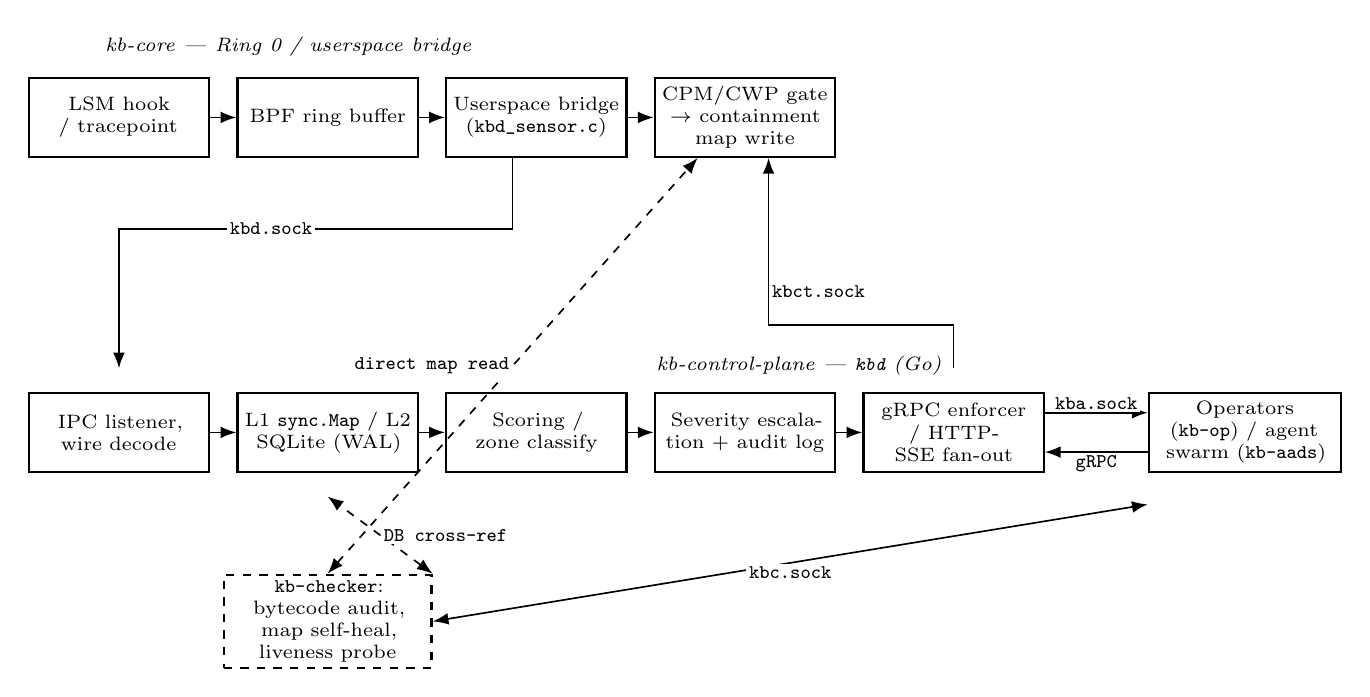
\begin{tikzpicture}[
  stg/.style={draw, thick, minimum height=1.0cm, text width=2.15cm,
    align=center, font=\scriptsize, inner sep=2pt},
  lane/.style={font=\scriptsize\itshape},
  sock/.style={font=\scriptsize\ttfamily, fill=white, inner sep=1pt},
  >=Latex, line width=0.6pt, color=black
]
\node[lane, anchor=west] at (-0.3,3.9) {kb-core --- Ring 0 / userspace bridge};
\node[stg] (h1) at (0,3)   {LSM hook / tracepoint};
\node[stg] (h2) at (2.65,3) {BPF ring buffer};
\node[stg] (h3) at (5.3,3)  {Userspace bridge (\texttt{kbd\_sensor.c})};
\node[stg] (h4) at (7.95,3) {CPM/CWP gate $\to$ containment map write};

\draw[->] (h1) -- (h2);
\draw[->] (h2) -- (h3);
\draw[->] (h3) -- (h4);

\node[lane, anchor=west] at (6.7,-0.15) {kb-control-plane --- \texttt{kbd} (Go)};
\node[stg] (c1) at (0,-1)    {IPC listener, wire decode};
\node[stg] (c2) at (2.65,-1) {L1 \texttt{sync.Map} / L2 SQLite (WAL)};
\node[stg] (c3) at (5.3,-1)  {Scoring / zone classify};
\node[stg] (c4) at (7.95,-1) {Severity escalation + audit log};
\node[stg] (c5) at (10.6,-1) {gRPC enforcer / HTTP-SSE fan-out};

\draw[->] (c1) -- (c2);
\draw[->] (c2) -- (c3);
\draw[->] (c3) -- (c4);
\draw[->] (c4) -- (c5);

\node[stg, text width=2.3cm] (consumers) at (14.3,-1) {Operators (\texttt{kb-op}) / agent swarm (\texttt{kb-aads})};
\draw[->] ([yshift=2.5mm]c5.east) -- node[sock, above]{\texttt{kba.sock}} ([yshift=2.5mm]consumers.west);
\draw[->] ([yshift=-2.5mm]consumers.west) -- node[sock, below]{gRPC} ([yshift=-2.5mm]c5.east);

\draw[->] ([xshift=-3mm]h3.south) -- ++(0,-0.9) -| node[pos=0.25, sock, left]{\texttt{kbd.sock}} ([yshift=3mm]c1.north);
\draw[->] ([yshift=3mm]c5.north) -- ++(0,0.55) -| node[pos=0.6, sock, right]{\texttt{kbct.sock}} ([xshift=3mm]h4.south);

\node[stg, text width=2.5cm, dashed] (checker) at (2.65,-3.4) {\texttt{kb-checker}: bytecode audit, map self-heal, liveness probe};
\draw[<->, dashed] (checker.north) -- node[sock, left]{direct map read} ([xshift=-6mm]h4.south);
\draw[<->, dashed] (checker.north east) -- node[sock, right]{DB cross-ref} ([yshift=-3mm]c2.south);
\draw[<->] (checker.east) -- node[sock, below]{\texttt{kbc.sock}} ([yshift=-4mm]consumers.south west);
\end{tikzpicture}
\caption{Socket topology traced to internal pipeline stages, not just
socket ownership (contrast \Cref{tab:sockets}). Solid arrows within a
lane are in-process control/data flow (function calls, eBPF ring-buffer
submit/consume); solid arrows crossing a lane boundary are the labeled
Unix domain socket. Dashed arrows are \texttt{kb-checker}'s independent,
out-of-band verification paths (\S\ref{sec:checker}) --- it reads
kernel state and the L2 database directly to cross-check them, rather
than trusting either side's own report of itself.}
\label{fig:pipeline}
\end{figure*}

\section{Feature Set}
\label{sec:features}

\Cref{tab:features} summarizes the implemented feature set by
subsystem and status, consolidating features discussed in detail in
their respective sections. ``Live-verified'' means the feature was
exercised against a running instance of the relevant component (not
only a unit test in isolation) during this project's development;
``proposed'' means design-only, with no code.

\begin{table}[htbp]
\centering
\footnotesize
\caption{Feature set by subsystem, condensed. See referenced sections
for detail.}
\label{tab:features}
\begin{tabular}{@{}p{1.9cm}p{3.9cm}p{1.1cm}@{}}
\toprule
Subsystem & Feature & Status \\
\midrule
\multirow{5}{*}{\parbox{1.9cm}{\texttt{kb-core}}}
 & 5-level containment (\S\ref{sec:core}) & Verified \\
 & CPM / CWP gates (\S\ref{sec:core}) & Verified \\
 & Rate limiting (\S\ref{sec:core}) & Verified \\
 & socket split (\S\ref{sec:core-split}) & Verified \\
 & CO-RE/BTF portability & Done \\
\midrule
\multirow{6}{*}{\parbox{1.9cm}{\raggedright\texttt{kb-control-\\plane}}}
 & L1/L2 storage (\S\ref{sec:storage}) & Verified \\
 & Audit log (\S\ref{sec:audit-log}) & Verified \\
 & Policy hot-reload (\S\ref{sec:policy-reload}) & Verified \\
 & Signed CWP policy (\S\ref{sec:cwp-sign}) & Verified \\
 & Severity escalation (\S\ref{sec:severity}) & Verified \\
 & Exfiltration detection (\S\ref{sec:exfil}) & Verified \\
\midrule
\multirow{7}{*}{\parbox{1.9cm}{\texttt{kb-aads}}}
 & Containment RL (\S\ref{sec:rl}) & Verified \\
 & Jury RL (\S\ref{sec:jury-rl}) & Verified \\
 & Patroller / Healer (\S\ref{sec:patroller-healer}) & Verified \\
 & Militia (\S\ref{sec:militia}) & Verified \\
 & Signal relays (\S\ref{sec:militia}) & Verified \\
 & Registry + courthouse (\S\ref{sec:courthouse}) & Verified \\
 & Hunter logic & Stub \\
\midrule
\multirow{3}{*}{\parbox{1.9cm}{\texttt{kb-checker}}}
 & Integrity/self-heal (\S\ref{sec:checker}) & Verified \\
 & Liveness audit (\S\ref{sec:checker}) & Verified \\
 & Boot gating (\S\ref{sec:checker}) & Verified \\
\midrule
\multirow{4}{*}{\parbox{1.9cm}{\texttt{kb-op}}}
 & \texttt{kbctl} CLI (\S\ref{sec:op}) & Verified \\
 & \texttt{kb-tui} console (\S\ref{sec:op}) & Verified \\
 & \texttt{kb-dashboard} (\S\ref{sec:op}) & Verified \\
 & \texttt{kb-mcp} server & Not audited \\
\bottomrule
\end{tabular}
\end{table}

\section{Mathematical Formulation}
\label{sec:math}

This section collects every learned or statistically-driven decision
rule in KB in one place. Each subsection restates, briefly, where the
rule is used; the corresponding system section gives full context.

\subsection{Containment Level Selection (Reinforcement Learning)}
\label{sec:math-containment}

Containment's decision (\S\ref{sec:rl}) is a single-step Markov
Decision Process over a 5-dimensional observation
$o = (\mathrm{score}, \mathrm{zone}, u_{\mathrm{root}}, \Delta_{\mathrm{score}}, e) \in \mathbb{R}^5$,
a 5-way discrete action $a \in \{0,1,2,3,4\}$ matching
\texttt{ContainmentLevel} (\texttt{NONE} through \texttt{TERMINATE}),
and reward
\begin{equation}
  r(a, t) = 1 - 0.3\,|a-t| - 0.2\,|a-t|\cdot\mathbb{1}[a < t]
  \label{eq:containment-reward}
\end{equation}
against a labeled target level $t$, penalizing under-containment
($a<t$) more heavily than over-containment. The policy is a PPO
actor \citep{schulman2017proximal} trained via RLlib
\citep{liang2018rllib} on Ray \citep{moritz2018ray}; inference at
serving time is $a^\ast = \arg\max_a \pi_\theta(a \mid o)$, taken from
the policy's action-distribution logits with no exploration noise.

\subsection{Jury Vote Selection (Reinforcement Learning)}
\label{sec:math-jury}

Jury's decision (\S\ref{sec:jury-rl}) reuses Containment's exact
observation space $o \in \mathbb{R}^5$ and dataset, coarsened to a
binary target
$t' = \mathbb{1}[t > 0]$ (any nonzero containment level $\Rightarrow$
CONTAIN). The action space is $a' \in \{\text{ALLOW}, \text{CONTAIN}\}$
and the reward, matching \texttt{kb-aads}'s pre-existing reward-signal
table, is
\begin{equation}
  \small
  r'(a', t') =
  \begin{cases}
    +1.0 & a'\!=\!\text{CONTAIN},\ t'\!=\!\text{CONTAIN}\ \text{(TP)}\\
    -0.5 & a'\!=\!\text{CONTAIN},\ t'\!=\!\text{ALLOW}\ \text{(FP)}\\
    +0.1 & a'\!=\!\text{ALLOW},\ t'\!=\!\text{ALLOW}\ \text{(TN)}\\
    -1.0 & a'\!=\!\text{ALLOW},\ t'\!=\!\text{CONTAIN}\ \text{(FN)}
  \end{cases}
  \normalsize
  \label{eq:jury-reward}
\end{equation}
Where a full observation vector is unavailable, Jury falls back to a
fixed-threshold rule on a bare confidence scalar $c \in [0,1]$,
\begin{equation}
  \mathrm{vote}(c) = \begin{cases}\text{CONTAIN} & c > 0.75\\ \text{ALLOW} & \text{otherwise}\end{cases}
  \label{eq:jury-fallback}
\end{equation}
which is the path every caller in the system uses today (\S\ref{sec:jury-rl}).

\subsection{JJE Quorum Consensus}
\label{sec:math-quorum}

Given a set of $n$ weighted votes $\{(v_i, w_i)\}_{i=1}^n$ from a
dynamically-spawned Jury pool, $v_i \in \{\text{CONTAIN}, \text{ALLOW}\}$,
quorum for containment is reached iff
\begin{equation}
  \frac{\sum_{i: v_i = \text{CONTAIN}} w_i}{\sum_{i=1}^n w_i} > \tfrac12,
  \label{eq:quorum}
\end{equation}
defined as false on $n=0$ (every juror in the round failed) rather
than raising a division error. In the current implementation every
$w_i = 1.0$ (unweighted majority); the formula is written in weighted
form because the wire format already carries a per-vote weight field.

\subsection{Beaconing Detection: Timing Entropy}
\label{sec:math-entropy}

For a sliding window of the most recent $\min(N,100)$ inter-connection
intervals $\{\Delta t_1,\dots,\Delta t_N\}$ for one (pid, destination
address, destination port) flow, each interval is binned into one of
five fixed buckets $B = \{(0,1], (1,5], (5,10], (10,30], (30,\infty)\}$
seconds, and Shannon entropy \citep{shannon1948mathematical} is
computed over the resulting empirical bin distribution $p_j = n_j / N$:
\begin{equation}
  H = -\sum_{j=1}^{5} p_j \log_2 p_j.
  \label{eq:entropy}
\end{equation}
$H \to 0$ indicates high timing regularity (a rigid periodic timer,
characteristic of a beacon); $H$ is undefined below ten samples and a
sentinel value of $3.0$ (``unprofiled, treat as high/benign'') is
returned instead. The detector's default beacon threshold is
$H < 1.2$.

\subsection{Slow-Exfiltration Detection: CUSUM over Connection Rate}
\label{sec:math-cusum}

For the same flow, connection events are aggregated into fixed
60-second buckets; let $x_i$ be the connection count in bucket $i$. A
running mean $\mu_i$ and variance are maintained online via Welford's
algorithm (no raw history retained):
\begin{align}
  \delta_i &= x_i - \mu_{i-1}, \qquad
  \mu_i = \mu_{i-1} + \frac{\delta_i}{i}, \\
  M_{2,i} &= M_{2,i-1} + \delta_i\,(x_i - \mu_i), \qquad
  \sigma_i = \sqrt{\frac{M_{2,i}}{i-1}}.
\end{align}
A one-sided upper CUSUM statistic \citep{page1954continuous} is then
updated with slack $k = \sigma_i / 2$:
\begin{equation}
  S_i = \max\!\big(0,\; S_{i-1} + (x_i - \mu_i - k)\big),
  \label{eq:cusum}
\end{equation}
and flagged once $S_i > 5\sigma_i$, meaningful only once at least five
buckets have closed (an early verdict off a near-empty baseline would
be noise, not signal). An \texttt{EXFIL\_BEACON\_SUSPECTED} alert fires
only when \emph{both} $H < 1.2$ \emph{and} $S_i > 5\sigma_i$ hold
simultaneously for the same flow, combining a fine-grained timing
signal with a coarser volume-shift signal specifically to suppress the
false positives either alone would produce, and is debounced to at
most one alert per flow per five minutes. This implementation's own
stated fidelity limitation: $x_i$ is a connection-frequency proxy, not
true byte volume, since \texttt{kb-core}'s \texttt{connect()} telemetry
carries no payload-size field (\S\ref{sec:exfil}).

\subsection{CWP Severity Escalation}
\label{sec:math-severity}

A raw composite score $s \in [0,100]$ (already computed upstream by the
Behavior Engine, not re-derived here) is bucketed into one of four
ordered tiers by
\begin{equation}
  \mathrm{tier}(s) = \begin{cases}
    \text{CRITICAL} & s \geq 90 \\
    \text{HIGH} & 75 \leq s < 90 \\
    \text{MEDIUM} & 50 \leq s < 75 \\
    \text{LOW} & s < 50
  \end{cases}
  \label{eq:severity}
\end{equation}
and escalated exactly one tier, capped at CRITICAL, when the alerting
process's executable basename matches a registered Critical Workload
Protection (CWP) entry (\S\ref{sec:severity}). This basename match is
an explicitly documented, lower-stakes trade-off for alert routing
only --- the actual containment-exemption decision uses \texttt{kb-core}'s
kernel-side path-resolved match (\S\ref{sec:core}), unaffected by this
rule.

\subsection{JJE Courthouse Severity Ladder}
\label{sec:math-courthouse}

For a registered sub-agent, let $e$ be its cumulative
\texttt{error\_count}, $\sigma \in \{\text{active}, \neg\text{active}\}$
its reported status, and $u_0, u_1$ its uptime read before and after a
liveness window of length $\tau$ (default $3$s). The courthouse
classifier (\S\ref{sec:courthouse}) is
\begin{equation}
  \small
  \mathrm{severity} = \begin{cases}
    \text{terminate} & \text{agent unregistered} \\
    \text{restart} & \sigma \!\neq\! \text{active} \ \lor\ e \!\geq\! \theta_e \ \lor\ u_1 \!\leq\! u_0 \\
    \text{healthy} & \text{otherwise}
  \end{cases}
  \normalsize
  \label{eq:courthouse}
\end{equation}
with default error-count threshold $\theta_e = 5$. The classifier never
automatically returns \texttt{revoke} or (for a still-registered agent)
\texttt{terminate} --- those tiers require a peer-baseline
output-drift signal and an authorization-boundary-violation signal
respectively, neither of which this codebase currently computes
(\S\ref{sec:courthouse}); \Cref{eq:courthouse} is stated exactly as
implemented, not as the ladder's eventual full form.

\subsection{Audit Log Integrity}
\label{sec:math-audit}

Each audit row $i$ commits to every prior row via a SHA-256 hash chain,
\begin{equation}
  h_i = \mathrm{SHA256}(f_i \,\|\, h_{i-1}), \qquad h_0 = \mathbf{0},
  \label{eq:hashchain}
\end{equation}
where $f_i$ is the row's serialized field tuple. Mutating or deleting
any row $j < i$ changes $h_j$ and therefore every $h_k$ for $k \geq j$
under the second-preimage resistance of SHA-256, making a chain break
detectable by recomputing \Cref{eq:hashchain} end to end
(\S\ref{sec:audit-log}).

\section{kb-core: eBPF Sensor and Enforcement Primitives}
\label{sec:core}

\texttt{kb-core} is a C/eBPF subsystem, built with CO-RE (Compile Once,
Run Everywhere) via BTF for cross-kernel portability without
per-kernel-version recompilation. It is the only subsystem with a
presence in Ring 0. A full \texttt{make} of \texttt{kb-core}, including
eBPF bytecode compilation for every collector
(\texttt{kb\_process}, \texttt{kb\_syscall}, \texttt{kb\_privilege},
\texttt{kb\_file}, \texttt{kb\_network}, \texttt{kb\_memory}) and the
combined \texttt{kbd\_sensor} binary, was verified clean at the time of
writing.

\subsection{Hook Points and the Containment Model}

\texttt{kb-core} attaches LSM hooks and tracepoints covering process
execution (\texttt{bprm\_check\_security}), file access
(\texttt{file\_open}), network connect/bind, memory-protection changes
(\texttt{file\_mprotect}), and credential changes
(\texttt{commit\_creds}), and maintains a five-level containment state
per monitored process, uniform across all hooks, escalating through the
standard Linux primitives of cgroups, seccomp, and namespaces
\citep{kerrisk2010linux}:
\texttt{NONE} (no entry; every hook passes through), \texttt{CGROUP}
(resource throttling only, no LSM blocking), \texttt{SECCOMP} (blocks
new network connections/binds and process exec), \texttt{NAMESPACE}
(adds RWX/exec memory-protection blocking on top of \texttt{SECCOMP}),
and \texttt{TERMINATE} (blocks everything interceptable, combined with
a userspace \texttt{SIGKILL} as a belt-and-suspenders measure). Every
hook returns a uniform \texttt{-EPERM} rather than hook-specific error
codes, so the kernel presents a consistent ``Operation not permitted''
regardless of which containment layer intervened.

\subsection{CPM and CWP: Authorization Gates on Containment Writes}
\label{sec:cpm-cwp}

Two authorization layers sit in front of containment map writes, both
implemented in userspace C (\texttt{kbd\_sensor.c}'s
\texttt{cpm\_classify()}/\texttt{cwp\_classify()}) rather than in-kernel
eBPF --- a deliberate, documented deviation from an earlier design
sketch, since the real last-gate-before-enforcement choke point in this
codebase is \texttt{handle\_incoming\_containment\_cmd()}, itself
userspace. \textbf{CPM (Critical Process Module)}
(\Cref{alg:cpm}) refuses to contain PID 1, kernel threads (detected by
a failed \texttt{/proc/\textless pid\textgreater/exe} readlink), any
PID in \texttt{protected\_pids\_map}, or any process whose live-resolved
executable path matches \texttt{protected\_exec\_paths\_map} --- the
last check exists specifically as a race-safety net against a
just-executed protected binary not yet reflected in the PID map. Its
compiled-in floor (\texttt{populate\_protected\_exec\_paths()}) now
covers \texttt{systemd}, \texttt{dbus-daemon}, \texttt{NetworkManager},
\texttt{kb-checker}, \texttt{kbd}, \texttt{kbagents}, \texttt{kbopd},
and \texttt{kbopt} --- closing a prior gap where KB's own watchdog or
policy engine could in principle be recommended for containment through
KB's own pipeline. Both backing maps are marked
\texttt{BPF\_F\_RDONLY\_PROG} so no in-kernel BPF program can write
either, only userspace, and \texttt{protected\_pids\_map} entries are
populated at exec time and cleared at exit time so a reused PID cannot
inherit a predecessor's protection.

\textbf{CWP (Critical Workload Protection)} (\Cref{alg:cwp}) is
evaluated strictly after CPM returns allow, never merged with it. Each
registered workload carries a single \texttt{identity\_tier} byte, not
two independent lookup mechanisms: \texttt{PATH} tier rejects on a bare
path/PID match, while \texttt{HASH} tier defers to a SHA-256 content
check computed at decision time (hashing cannot happen in-kernel;
registration only stores the tier flag and expected digest). A hash
\emph{mismatch} on a \texttt{HASH}-tier entry does not itself block
anything --- it logs a distinct ``Identity Verification Failed'' security
event and falls through to ordinary containment eligibility, since the
process is thereby confirmed \emph{not} to be the protected workload it
claimed to be. \texttt{protected\_workloads\_map} is sized to 8192
entries with no compiled-in floor, since protected workloads are
organization-specific by design. Both gates were verified against the
live running sensor, not merely built: a live test confirmed that a
containment command for a protected PID was rejected correctly while
the connection was simultaneously saturated with unrelated telemetry.

\begin{algobox}{CPM classification (\texttt{cpm\_classify}, \texttt{kbd\_sensor.c:677--702})}
\label{alg:cpm}
1: if readlink(/proc/PID/exe) fails then\\
2: \quad return REJECT\_KERNEL\_THREAD\\
3: if PID = 1 then return REJECT\_PID1\\
4: if PID $\in$ protected\_pids\_map then\\
5: \quad return REJECT\_PROTECTED\_PID\\
6: path $\gets$ readlink(/proc/PID/exe)\\
7: if path $\in$ protected\_exec\_paths\_map then\\
8: \quad return REJECT\_PROTECTED\_EXEC\\
9: return ALLOW \quad(only reached if steps 1--8 all miss)
\end{algobox}

\begin{algobox}{CWP classification (\texttt{cwp\_classify}, \texttt{kbd\_sensor.c:964--1045})}
\label{alg:cwp}
1: tier $\gets$ lookup(protected\_workloads\_map, PID)\\
2: if tier not found then\\
3: \quad path $\gets$ readlink(/proc/PID/exe); if fails, return ALLOW\\
4: \quad tier $\gets$ lookup(protected\_workload\_paths\_map, path)\\
5: \quad if tier not found then return ALLOW\\
6: if tier = PATH then return REJECT\_PROTECTED\_PATH\\
7: \{tier = HASH\}: recompute path if not already resolved;\\
8: \quad if resolution fails then return REJECT\_PROTECTED\_HASH \quad(fail-closed)\\
9: entry $\gets$ registry lookup(path); if none, return REJECT\_PROTECTED\_HASH\\
10: digest $\gets$ SHA256(file contents at path)\\
11: if digest $\neq$ entry.expected\_hash then\\
12: \quad log(``Identity Verification Failed''); return ALLOW\\
13: else return REJECT\_PROTECTED\_HASH
\end{algobox}

\subsection{The kbd.sock / kbct.sock Split}
\label{sec:core-split}

Telemetry and containment commands were originally multiplexed on a
single, hand-rolled socket connection between the sensor and the
control plane. This proved to be a latent availability bug: a
telemetry-volume burst could fill the connection's send buffer,
\texttt{write()} would return \texttt{EAGAIN}, and the sensor's error
handling misread this as a dead connection and closed it --- taking
containment delivery down as collateral damage of an unrelated
telemetry spike. The fix splits control traffic (containment commands,
sensitive-path, rules, and CWP-workload pushes) onto a dedicated
\texttt{kbct.sock}, leaving \texttt{kbd.sock} telemetry-only, and
additionally ignores \texttt{SIGPIPE} process-wide so a closed peer
cannot kill the sensor via signal regardless of the split.

\subsection{Rate Limiting}
\label{sec:ratelimit}

Telemetry rate limiting (\Cref{alg:ratelimit}) uses a hybrid token
bucket per \texttt{\{tgid, start\_time, resource\_id\}} key in a
10240-entry BPF LRU hash map --- keying on the task's creation
timestamp alongside its tgid, not tgid and resource alone, specifically
to prevent a PID-reuse collision from inheriting a stale or already-
exhausted predecessor's bucket. Resource IDs are call-site specific:
the syscall number for generic syscall telemetry, a packed
\texttt{(daddr\textless\textless16)|dport} for network connect/bind,
and the relevant flag word for \texttt{mmap}/\texttt{mprotect} ---
specifically to prevent an evasion technique in which an attacker
distributes activity across many distinct resources to stay under a
single flat per-PID limit. Bucket capacity is 100 tokens, refilling at
one token per 10ms (100 tokens/second); a bucket that recovers tokens
after having dropped events emits one \texttt{KB\_EVT\_DROPPED\_
TELEMETRY} summary event carrying the suppressed count, rather than
silently discarding the fact that throttling occurred. Tier-1 events
--- privilege-escalation (\texttt{commit\_creds}), sensitive-capability
probes, and TLS-plaintext capture --- are exempted from throttling
structurally: their handlers simply never call the throttle function
before submitting to the ring buffer, not via a bypass flag. (LSM
enforcement hooks, \S\ref{sec:core}, have no corresponding telemetry
event at all on denial --- they return a kernel error code directly and
never touch the ring buffer or the rate limiter, so ``exempting'' a
denial from throttling is not applicable to them.)

\begin{algobox}{Token-bucket throttle (\texttt{kb\_rate\_limit\_throttle}, \texttt{kbd\_sensor.bpf.c:235--287})}
\label{alg:ratelimit}
1: key $\gets$ \{tgid, task.start\_time, resource\_id\}\\
2: bucket $\gets$ lookup(lru\_map, key)\\
3: if bucket = NULL then\\
4: \quad bucket $\gets$ \{tokens: 100, last: now, dropped: 0\}; insert\\
5: elapsed $\gets$ now $-$ bucket.last\\
6: if elapsed $>$ 10ms then\\
7: \quad bucket.tokens $\gets \min(100,\ \text{bucket.tokens} + \lfloor\text{elapsed}/\text{10ms}\rfloor)$\\
8: \quad bucket.last $\gets$ now\\
9: if bucket.dropped $>0$ and bucket.tokens $>0$ then\\
10: \quad emit DROPPED\_TELEMETRY(count = bucket.dropped); bucket.dropped $\gets 0$\\
11: if bucket.tokens $>0$ then bucket.tokens $\mathrel{-}= 1$; return ALLOW\\
12: else bucket.dropped $\mathrel{+}= 1$; return THROTTLE
\end{algobox}

\subsection{New Wire Message: Network-Flow Timestamps}

A new userspace-only wire message, \texttt{KB\_WIRE\_MSG\_NET\_FLOW}
(message type 9, a 22-byte \texttt{\{pid, daddr, dport, ts\_ns\}}
frame), is sent from \texttt{kbd\_sensor}'s existing
\texttt{KB\_EVT\_NETWORK\_CONNECT} handler to feed
\S\ref{sec:exfil}'s exfiltration detector. This required no eBPF or
kernel-side change --- the timestamp is already available in the
existing userspace event path, per the exfiltration-detection design's
own recommendation to avoid adding Ring-0 overhead for a control-plane
statistical computation.

\subsection{Known Defects}

A historical, critical defect is documented here for completeness: an
early version of the sensitive-path LSM block was unconditional
(applied to every process, not only contained ones), and the first time
it fired correctly in the project's history it blocked
\texttt{/etc/sudoers}/\texttt{/etc/shadow} reads system-wide, breaking
\texttt{sudo}, \texttt{su}, \texttt{pkexec}, and login authentication
simultaneously on the test host, recoverable only via a full external
VM restart. This was fixed by making the block containment-gated,
consistent with every other hook. A related bug --- the block
technically never enforced anything even when intended to, because
\texttt{bpf\_d\_path()} does not zero the tail of its output buffer
past the NUL terminator, causing exact-match lookups against a
fixed-size key to silently fail --- was found and fixed by explicitly
zero-filling the buffer. An earlier revision of this paper's audit
reported two further items as open that re-verification against
current source shows are already resolved: \texttt{kb\_lsm\_file\_open}
checks the level-3+ block \emph{before} resolving the path via
\texttt{bpf\_d\_path()} (\Cref{alg:cpm}'s sibling hook, same file), so a
path-resolution failure cannot bypass full quarantine; and of the two
genuinely PID-keyed telemetry maps (\texttt{kb\_syscall\_totals},
\texttt{kb\_cred\_prev}), both are explicitly deleted in
\texttt{kb\_handle\_exit}. A third map,
\texttt{kb\_syscall\_counts}, is composite-keyed
(\texttt{pid<<32|syscall\_nr}) rather than PID-keyed, so a single-PID
delete on exit cannot target its entries without iterating the whole
map; it uses \texttt{BPF\_MAP\_TYPE\_LRU\_HASH} instead, which ages out
old entries under normal churn --- a different, and adequate, mitigation
for the same exhaustion concern, not an oversight.

\section{kb-control-plane: Scoring, Storage, and Enforcement}
\label{sec:cp}

\texttt{kb-control-plane} is a Go daemon (\texttt{kbd}) responsible for
ingesting sensor telemetry, maintaining process state, exposing a gRPC
and HTTP API, and issuing containment commands back to the sensor. Its
Go test suite --- \texttt{internal/audit}, \texttt{controlplane},
\texttt{detection}, \texttt{enforcement}, \texttt{ipc}, \texttt{policy},
\texttt{store} --- comprises 128 passing tests with zero failures at
the time of writing.

\subsection{Storage: L1/L2 Hybrid}
\label{sec:storage}

State is kept in a two-layer store, per this project's ADR-1: an
in-memory \texttt{sync.Map} (L1), authoritative for all reads, and an
asynchronously-written SQLite database in WAL mode (L2), durable and
single-writer (\texttt{SetMaxOpenConns(1)}) via a buffered channel, so
that L1 writers never block on disk I/O even under load. On startup, L1
is restored from L2's durable copy. PID-reuse safety is handled
explicitly: a process-exit wire message flushes both the stale L1 entry
and the L2 row immediately, so a later, unrelated process reusing the
same PID cannot inherit a predecessor's cached state.

\subsection{The Audit Log}
\label{sec:audit-log}

Every enforcement action, policy reload, and agent decision is recorded
in a SHA-256 hash-chained append-only log (\Cref{eq:hashchain},
\Cref{alg:auditchain}): each row's \texttt{entry\_hash} commits to that
row's own fields joined with the \emph{previous} row's
\texttt{entry\_hash} (\texttt{prev\_hash}) --- the chain runs through
\texttt{prev\_hash}, not through a row hashing its own
\texttt{entry\_hash} recursively --- rooted at the literal genesis
value \texttt{"genesis"}. A \texttt{VerifyChain()} routine existed
correctly for some time before being wired to anything callable
outside its own test --- meaning the security property existed in code
but delivered no operational value until an HTTP route
(\texttt{GET /api/audit/verify}) and a gRPC \texttt{VerifyAuditChain}
method were added to actually invoke it, alongside a
\texttt{kbctl audit verify} command (\S\ref{sec:op}). This audit's own
review of \texttt{VerifyChain()} found a real defect in exactly the
direction that matters most for a security property: after its
row-iteration loop exits, it never calls Go's \texttt{rows.Err()}.
\texttt{sql.Rows.Next()} returns \texttt{false} both on ordinary
exhaustion \emph{and} on an underlying driver/I/O error mid-cursor, with
the real error stashed on \texttt{rows.Err()} rather than returned by
\texttt{Next()} itself --- so a genuine I/O error partway through
verification is silently indistinguishable from a clean, complete scan,
and \texttt{VerifyChain()} reports the chain valid (\texttt{true}) with
a row count lower than the true total, rather than surfacing the
error. This is a false-confidence bug, not a false-alarm one: it can
under-report tampering exposure by claiming a shorter, unverified
prefix is the whole story, not incorrectly flag an intact chain as
broken. Fixed in this revision by checking \texttt{rows.Err()}
immediately after the loop and returning it as a genuine failure rather
than falling through to the success path (\Cref{alg:auditchain}), with
a dedicated regression test using a fault-injecting
\texttt{database/sql/driver} wrapper that fails the cursor mid-scan ---
a scenario the existing test suite's row-\texttt{Scan}-error test
(itself a distinct, already-correctly-handled case) did not cover.

\begin{algobox}{Audit chain log/verify (\texttt{internal/audit/audit.go})}
\label{alg:auditchain}
\textbf{Log}(ts, action, subject, actor, reason):\\
1: content $\gets$ ts $\|$ action $\|$ subject $\|$ actor $\|$ reason $\|$ prev\_hash\\
2: entry\_hash $\gets$ SHA256(content)\\
3: append row; prev\_hash $\gets$ entry\_hash\\[4pt]
\textbf{VerifyChain}():\\
4: rows $\gets$ SELECT * FROM audit\_log ORDER BY id ASC\\
5: if query error then return (false, 0, err)\\
6: prev $\gets$ "genesis"; count $\gets 0$\\
7: while rows.Next() do\\
8: \quad if scan error then return (false, count, err)\\
9: \quad expected $\gets$ SHA256(row fields $\|$ prev)\\
10: \quad if expected $\neq$ row.entry\_hash then\\
11: \qquad return (false, count, "chain broken")\\
12: \quad prev $\gets$ row.entry\_hash; count $\mathrel{+}= 1$\\
13: \textcolor{teal}{if rows.Err() $\neq$ nil then return (false, count, err)} \quad\textcolor{teal}{\{fix\}}\\
14: return (true, count, nil)
\end{algobox}

\subsection{Policy Engine and Hot-Reload}
\label{sec:policy-reload}

\texttt{policy.yaml} configures per-process auto-terminate overrides
and the sensitive-paths list consulted by \texttt{kb-core}. Changing
this configuration originally required a full daemon restart, which
also dropped every sensor connection and forced a cold-start L1
rebuild. This was corrected by adding a \texttt{ReloadPolicy} gRPC
method that re-reads \texttt{policy.yaml} and atomically swaps a freshly
built \texttt{policy.Engine} into place under a \texttt{sync.RWMutex}
--- a full lock on the (rare) write path, a read lock on the (frequent,
per-zone-transition) read path --- verified during this audit to be
genuinely race-free. A separate, previously-diagnosed-backwards
misconfiguration is worth recording precisely because the first
diagnosis was wrong: \texttt{kb-control-plane/config/policy.yaml} (the
file \texttt{kbd}'s default \texttt{--policy} flag resolves to when run
from its own documented working directory) carried the old,
pre-\texttt{internal/policy} schema and silently produced empty,
unenforced policies with no error --- while the root-level
\texttt{config/policy.yaml} was, and had always been, correctly
schema-conformant. This was confirmed empirically (not by inspection)
by running \texttt{policy.New} against both files directly, and fixed
by replacing the daemon-default file's content to match.

\subsection{Signed Critical-Workload Policy}
\label{sec:cwp-sign}

Critical Workload Protection's local policy file, \texttt{workloads.yaml},
can now be signed: \texttt{SignWorkloadsFile}/\texttt{VerifyWorkloadsSignature}
implement Ed25519 signing over a deterministic JSON serialization of
the file's \texttt{critical\_workloads} and \texttt{policy\_metadata}
content, excluding the signature field itself. Passing
\texttt{kbd --workloads-pubkey <path>} makes verification mandatory: a
missing, invalid, or tampered signature is rejected outright and the
previous known-good registry is retained rather than partially
trusted. \texttt{kbctl workload keygen}/\texttt{sign} give operators an
actual signing workflow; because \texttt{kbctl} is a separate Go module
from \texttt{kb-control-plane}, its signing logic is a small,
intentionally self-contained mirror of the control plane's own
implementation --- Go's internal-package visibility rule blocks a
cross-module import of \texttt{kb-control-plane/internal/ipc}
regardless of the module's own \texttt{replace} directive, confirmed by
testing the import directly rather than assumed. What this closes is
local, host-resident policy signing; a networked central policy store
(a separate, documented specification section) is explicitly not
implemented, since no fleet-management server exists anywhere in this
codebase for any subsystem.

\subsection{CWP Severity Escalation}
\label{sec:severity}

Alerts arising from a BORDERLANDS-zone transition are now bucketed
into one of four severity tiers by raw score (\Cref{eq:severity})
rather than the previous behavior of always reporting ``CRITICAL''
regardless of actual severity, and escalated one tier when the
alerting process's executable basename matches a registered CWP
workload. The Go-side match is explicitly, and only, a basename match
against \texttt{comm} (a 16-byte wire field) --- the canonical,
path-resolved, spoofing-resistant match required for the actual
containment-exemption decision happens kernel-side in
\texttt{cwp\_classify()} and is unaffected; this Go-side rule governs
only alert severity and routing metadata
(\texttt{protected\_workload}/\texttt{owner\_team}/\texttt{justification}/
\texttt{policy\_id}, four new \texttt{Alert} proto fields).

\subsection{Exfiltration and Beaconing Detection}
\label{sec:exfil}

Implements the timing-entropy and CUSUM statistics of
\Cref{sec:math-entropy,sec:math-cusum} against the new
\texttt{KB\_WIRE\_MSG\_NET\_FLOW} stream. An
\texttt{EXFIL\_BEACON\_SUSPECTED} alert fires only when both signals
agree, debounced to one alert per (pid, destination address,
destination port) flow per five minutes --- without this debounce, a
sustained real beacon would re-alert and re-write an audit-log entry on
every single subsequent connection indefinitely, a bug caught by a
dedicated regression test before this shipped. Automatic
\texttt{NAMESPACE}-level containment on a confirmed beacon is available
but opt-in per process name via a new policy key,
\texttt{auto\_namespace\_on\_exfil\_beacon} (default \texttt{false}),
reflecting the same conservative default already applied to
\texttt{auto\_terminate} --- a statistical heuristic carries real
false-positive risk and should not silently gain enforcement authority
by default.

\subsection{Known Defects}

A historical, critical defect: the wire-level constant for containment
commands (\texttt{MsgTypeContainmentCmd}) was \texttt{3} on the Go side
but the C sensor checked for \texttt{5}, so every containment command
issued via any operator interface was silently dropped, while the
control plane's own audit log recorded a successful entry regardless
(the sensor never NACKs) --- completely masking the failure until a live
test against the running sensor exposed it. An earlier revision of this
paper's audit additionally reported five items as open that, on
re-verification directly against current source for this revision, are
already fixed in prior team history and were simply never re-checked
before being written up: the HTTP isolate/restore API now requires a
bearer token (\texttt{KB\_HTTP\_API\_TOKEN}, constant-time compared,
fails closed if unconfigured) and CORS is an explicit origin allowlist,
not a wildcard; \texttt{UpsertProcessState} explicitly preserves an
active PID's containment level across routine telemetry updates rather
than overwriting it; \texttt{SetContainment}/\texttt{SubmitAgentDecision}
both have existence checks and per-agent call throttling, covered by
dedicated tests; and the dashboard resolves its API host from
\texttt{window.location.hostname} (overridable via
\texttt{VITE\_KB\_API\_BASE}), not a hardcoded
\texttt{localhost:8080}. The audit-chain verifier's \texttt{rows.Err()}
gap (\S\ref{sec:audit-log}) was confirmed genuinely open and is fixed
in this revision (\Cref{alg:auditchain}), with a dedicated
fault-injecting-driver regression test.

\section{kb-aads: The Agent Defense Swarm}
\label{sec:aads}

\texttt{kb-aads} is a Python subsystem built on Ray, organized as a set
of role-specialized actors intended to jointly monitor, investigate,
and respond to threats. Its test suite comprises 68 passing tests
across eight agent-role modules at the time of writing.

\subsection{Actor Architecture}

Roles are implemented as Ray actors subclassing a common
\texttt{BaseAgent}: \textbf{Patroller} (baseline monitoring),
\textbf{Hunter} (threat investigation), \textbf{Healer} (recovery
decisions), \textbf{Containment} (enforcement-level selection),
\textbf{Containment militia} (mechanical escalation execution,
\S\ref{sec:militia}), \textbf{signal relays} (message dispatch,
\S\ref{sec:militia}), and a \textbf{Judge/Jury/Executor (JJE)}
consensus mechanism gating high-stakes decisions behind a quorum vote
(\Cref{eq:quorum}) before \textbf{Executor} carries them out over gRPC
to \texttt{kb-control-plane}. The actor scaffolding itself required a
non-trivial fix early in its development: \texttt{BaseAgent} was
originally decorated \texttt{@ray.remote} directly, which raises
\texttt{ActorClassInheritanceException} the instant any concrete role
subclass also applies \texttt{@ray.remote}. The fix removes the
decorator from the base class and applies it individually per concrete
subclass, with a \texttt{RemoteBaseAgent} convenience wrapper for roles
with no dedicated subclass.

\subsection{JJE Consensus}
\label{sec:jje}

Judge opens a round when a Patroller-raised alert crosses a threshold,
a dynamically-spawned Jury pool casts weighted votes
(\Cref{eq:quorum}), and Executor carries out the resulting decision
only after quorum. Two defects previously reported against this
mechanism are, at the time of writing, confirmed fixed in the current
source rather than open: Jury's vote threshold now correctly operates
on the same $[0,1]$ confidence scale used everywhere else in the system
(\Cref{eq:jury-fallback}, not the previously-reported unreachable
$75.0$ threshold against a $0$--$1$ input), and \texttt{coordinate\_
consensus}'s Jury pool size is read from \texttt{config/agents.yaml}
(\texttt{jury.pool\_size}) rather than hardcoded, confirmed by a
dedicated test asserting the exact spawn count for a configured value.
A crashed juror's exception is caught via
\texttt{asyncio.gather(..., return\_exceptions=True)}, so one failing
actor degrades the round's quorum computation rather than aborting it
entirely --- also confirmed by a dedicated test simulating two
crashing jurors out of three.

\begin{algobox}{JJE consensus round (\texttt{JudgeAgent.coordinate\_consensus})}
\label{alg:jje}
1: pool $\gets$ spawn $n$ = jury\_pool\_size fresh Jury actors\\
2: futures $\gets$ [jury.evaluate\_and\_vote(alert) for jury in pool]\\
3: results $\gets$ gather(futures, return\_exceptions = True)\\
4: votes $\gets$ [r for r in results if r is not Exception]\\
5: if votes is empty then return \quad(round skipped, no quorum)\\
6: if quorum\_reached(votes) $\{$\Cref{eq:quorum}$\}$ then\\
7: \quad executor.execute\_quarantine(alert)
\end{algobox}

\subsection{Containment: A Trained Reinforcement-Learning Policy}
\label{sec:rl}

Of \texttt{kb-aads}'s decision-making roles, Containment was the first
backed by a trained policy rather than a stub or an unreachable rule.
Applying reinforcement learning to intrusion response specifically (as
opposed to detection alone, the more heavily studied problem
\citep{liao2013intrusion}) is an active area;
we contribute a single, concrete, reproducible instance of it rather
than a general treatment, formulated in \Cref{sec:math-containment}.

\paragraph{Data.} No real eBPF-captured attack corpus existed for KB at
the time of this work, so real public data matching KB's actual
observation surface --- Linux syscall sequences, not network flow, which
an initially-tried NSL-KDD dataset was rejected for mismatching --- was
used instead. We mapped five of ADFA-LD's six attack categories
\citep{creech2013generation} onto five of KB's own
named attack scenarios (\Cref{tab:mapping}); KB's
\texttt{memory\_exploit} scenario has no ADFA-LD equivalent and is not
covered. The benign class combines ADFA-LD's Normal traces with real
\texttt{/proc}-derived telemetry sampled from a live development host.

\begin{table}[h]
\centering
\caption{ADFA-LD category to KB attack-scenario mapping.}
\label{tab:mapping}
\begin{tabular}{ll}
\toprule
ADFA-LD category & KB scenario \\
\midrule
Adduser & privilege\_escalation \\
Hydra\_FTP & credential\_access \\
Hydra\_SSH & lateral\_movement \\
Java\_Meterpreter & process\_injection \\
Meterpreter, Web\_Shell & reverse\_shell \\
\bottomrule
\end{tabular}
\end{table}

\paragraph{Training and a mid-training defect.} An initial PPO run
reached 97.8\% overall test accuracy but only 60--73\% on the
\texttt{CGROUP}/\texttt{SECCOMP} classes (\Cref{tab:run1}), root-caused
to \texttt{credential\_access} and \texttt{lateral\_movement} sharing
the same engineered \texttt{event\_type} code and \texttt{zone} floor.
Assigning each category a distinct code and retraining improved every
attack category to 97--100\% and reduced the under-containment rate to
0.0\%, at the cost of \texttt{NONE} accuracy falling from 100\% to
82.2\% (\Cref{tab:run2}) --- a trade we consider correct for a
containment system, since a false positive on benign traffic costs a
review action while a false negative on a real threat costs a missed
compromise.

\begin{table}[h]
\centering
\caption{Per-level test accuracy before and after the event\_type fix.}
\label{tab:run1}
\begin{tabular}{lrr}
\toprule
Level & Before fix & After fix \\
\midrule
NONE & 100.0\% & 82.2\% \\
CGROUP & 60.0\% & 100.0\% \\
SECCOMP & 70.4\% & 100.0\% \\
NAMESPACE & 100.0\% & 97.1\% \\
TERMINATE & 93.3\% & 100.0\% \\
\bottomrule
\end{tabular}
\end{table}

\begin{table}[h]
\centering
\caption{Overall test-set results before and after the fix.}
\label{tab:run2}
\begin{tabular}{lrr}
\toprule
& Before fix & After fix \\
\midrule
Overall accuracy & 97.8\% & 84.4\% \\
Under-containment rate & 1.1\% & \textbf{0.0\%} \\
\bottomrule
\end{tabular}
\end{table}

\paragraph{Live verification.} We verified the trained checkpoint three
ways: offline test-set evaluation (above); a direct unit-level check
against a live \texttt{ContainmentAgent} Ray actor for one synthetic
observation per attack scenario; and an end-to-end run streaming real
telemetry from KB's actual eBPF sensor and control plane on a live
host. The end-to-end check surfaced an integration defect distinct from
the model: the control plane returns a zero-value default
\texttt{ProcessState} (not an error) for an unscored PID, and a naive
feature mapping misread the resulting default \texttt{uid=0} as
``running as root,'' producing spurious high-severity decisions for
untracked, usually short-lived processes --- corrected by treating an
empty \texttt{comm} field as the true not-found signal.

\subsection{Jury: A Second Trained Policy}
\label{sec:jury-rl}

Jury's binary CONTAIN/ALLOW decision (\Cref{sec:math-jury}) is a strict
coarsening of Containment's own labeled question, so no new data
collection was needed: the identical \texttt{train.csv}/\texttt{val.csv}/
\texttt{test.csv} splits were reused with the target collapsed to
$t' = \mathbb{1}[t>0]$, and training used the same PPO/RLlib/Ray setup
as \Cref{sec:rl}. \Cref{tab:jury-results} reports held-out test
performance from the checkpoint currently on disk, re-run for this
revision rather than repeating an earlier session's unlogged figures
--- training uses no fixed random seed, so exact percentages vary
slightly run to run (an earlier run scored 99.8\%/99.4\% val/test on
the same splits); the qualitative result (near-perfect accuracy, zero
false negatives) has held across every run observed so far.

\begin{table}[h]
\centering
\caption{Jury policy held-out test results (908 samples), from the
checkpoint currently on disk.}
\label{tab:jury-results}
\begin{tabular}{lr}
\toprule
Metric & Value \\
\midrule
Validation accuracy & 100.0\% \\
Test accuracy & 100.0\% \\
CONTAIN recall & 100.0\% \\
False-negative rate & 0.0\% \\
\bottomrule
\end{tabular}
\end{table}

\texttt{JuryAgent.evaluate\_and\_vote} loads the resulting checkpoint
the same inference-only way \texttt{ContainmentAgent} does
(\texttt{RLModule.from\_checkpoint}, no training stack in the agent
process) and runs the trained policy only when a caller supplies a
full observation vector; every caller and test in the system today
supplies only a bare confidence scalar, so \Cref{eq:jury-fallback}'s
fixed-threshold rule remains the path actually exercised in practice
until a caller starts passing full observations --- stated plainly
rather than implied to be already in production use.

\subsection{Rule-Based Patroller and Healer}
\label{sec:patroller-healer}

Patroller previously set a static status string on every tick and took
no action; it now tracks a per-PID score and dispatches to a
round-robin Hunter pool (injected at construction, mirroring how Judge
receives its Executor reference) the moment a PID first crosses a
configurable suspicious-score threshold (default $40.0$), re-arming
once the score drops back below it. Healer's decision
(\S\ref{sec:jje}'s reward-table shape --- ``was un-containing this PID
actually safe?'') is \emph{not} reinforcement-learned, and this is a
stated, real gap rather than an oversight: that question needs
restore-\emph{outcome} ground truth (was the process actually safe $N$
minutes after restoration?), which does not exist anywhere in this
codebase --- Containment/Jury's training data has attack-\emph{category}
labels only, and the analyst-feedback loop that would eventually
produce restore-outcome labels remains undesigned. Healer instead
implements a genuine, conservative rule: restore only if zone is SAFE
\emph{and} score is below a safe threshold ($20.0$) \emph{and} a
minimum containment duration ($60$ ticks) has elapsed, with any
missing or ambiguous signal defaulting to the least permissive reading
(never accidentally \texttt{RESTORE}).

\subsection{Containment Militia and Signal Relays}
\label{sec:militia}

Two swarm roles previously existed only as design proposals, not code.
\textbf{Containment militia} implements the design's ``squad''
framing literally as an escalation sequence: a
\texttt{MilitiaSquadLeadAgent}, given a target containment level
$\ell \in \{1,\dots,4\}$ for one PID, spawns one mechanical
\texttt{MilitiaSquadMemberAgent} per stage
(\texttt{CGROUP}$\to$\texttt{SECCOMP}$\to$\texttt{NAMESPACE}$\to$
\texttt{TERMINATE}, matching Containment's own level ordering)
dynamically per incident --- mirroring Judge's own per-round Jury-pool
spawn pattern --- and executes them strictly in sequence via
\texttt{await}, so two stages can never race enforcement actions
against the same PID. Each member is genuinely mechanical: it calls
\texttt{ControlPlaneClient.set\_containment} for exactly the one stage
it owns, a real gRPC method that existed but had no live caller prior
to this work. Escalation halts on the first stage failure, with no
retry policy defined --- a stated, real gap rather than a silent
swallow. \textbf{Signal relays} implement the design's ``dedicated
messenger agent'' framing as a long-lived, tick-driven actor
round-robinning a message to a named destination pool, mirroring
Patroller's own pool-dispatch shape; one concrete route (to the Hunter
pool) is wired at swarm start, while other agent pairs continue to
call each other directly, an explicitly incomplete integration rather
than a claim that every message now flows through a relay.

\begin{algobox}{Militia escalation (\texttt{MilitiaSquadLeadAgent.command\_squad})}
\label{alg:militia}
1: stages $\gets$ [CGROUP, SECCOMP, NAMESPACE, TERMINATE][0{:}$\ell$]\\
2: for stage in stages do\\
3: \quad member $\gets$ spawn MilitiaSquadMemberAgent(stage)\\
4: \quad result $\gets$ await member.execute(pid, reason)\\
5: \quad \{blocking await: no two stages ever race on this pid\}\\
6: \quad if not result.success then\\
7: \qquad break \quad(halt; no retry policy defined)\\
8: return stage\_reports
\end{algobox}

\subsection{SwarmRegistry and JJE Courthouse Oversight}
\label{sec:courthouse}

The swarm's design calls for JJE to hold real authority to stop a
rogue sub-agent via a graduated restart/revoke/terminate response
(\Cref{eq:courthouse}), which required an actor-lookup mechanism that
did not previously exist: \texttt{RaySwarmOrchestrator}'s agent-handle
dictionary lives in the driver process, unreachable by a remote
\texttt{JudgeAgent}. A \texttt{SwarmRegistry} actor closes this gap;
registration happens at each spawn site (the orchestrator, Judge's
per-round Jury pool, the militia squad lead's per-stage members) rather
than via each agent self-registering inside its own \texttt{start()},
giving identical coverage of dynamically-spawned actors with no change
to \texttt{BaseAgent} or any existing agent subclass's constructor.
\texttt{JudgeAgent.assess\_severity} and \texttt{enforce\_verdict}
implement \Cref{eq:courthouse} and the corresponding mechanical
response (stop-then-restart on the same actor; stop plus mark-revoked
in the registry; \texttt{ray.kill} plus unregister), using two real,
newly-tracked signals --- a per-agent \texttt{error\_count} and a
genuine two-read liveness check. As \Cref{sec:math-courthouse} states
plainly, the classifier never automatically reaches \texttt{revoke} or
\texttt{terminate} for a still-live agent, since this codebase computes
no peer-baseline drift or authorization-boundary-violation signal; the
quorum-gating step the design calls for before acting on
restart/revoke is likewise not implemented, since forcing
\texttt{JuryAgent}'s existing threat-vote evaluator to answer a
structurally different question (``is this sub-agent rogue?'') via a
fabricated confidence input would not constitute a real vote.

\begin{algobox}{Courthouse verdict (\texttt{JudgeAgent.assess\_severity} + \texttt{enforce\_verdict})}
\label{alg:courthouse}
1: handle $\gets$ registry.get\_handle(agent\_id)\\
2: if handle = None then return TERMINATE\\
3: $s_0 \gets$ handle.get\_status()\\
4: if $s_0$.status $\neq$ active or $s_0$.error\_count $\geq \theta_e$ then\\
5: \quad return RESTART\\
6: sleep($\tau$); $s_1 \gets$ handle.get\_status()\\
7: if $s_1$.uptime $\leq s_0$.uptime then return RESTART\\
8: return HEALTHY\\[6pt]
\textbf{enforce\_verdict}(agent\_id, tier):\\
9: match tier:\\
10: \quad RESTART: handle.stop(); handle.start()\\
11: \quad REVOKE: handle.stop(); registry.revoke(agent\_id)\\
12: \quad TERMINATE: ray.kill(handle); registry.unregister(agent\_id)
\end{algobox}

\subsection{Status Note}

Hunter's investigation method remains an unimplemented stub (four bare
\texttt{TODO}s: query control-plane history, build an evidence chain,
compute confidence, submit to Jury) at the time of writing --- the one
swarm role, by design, intended to be a fine-tuned agentic LLM tool-call
loop rather than a rule or a numeric RL policy, and a substantially
larger, separate undertaking not attempted in this development cycle.

\section{kb-checker: Stateless Integrity Watchdog}
\label{sec:checker}

\texttt{kb-checker} is a Rust subsystem deliberately kept stateless and
network-free beyond its own local diagnostic socket, following a KISS
design principle intended to minimize its own attack surface as the
component responsible for detecting compromise of everything else.

\subsection{Active Auditing}

\texttt{kb-checker} performs three classes of active audit rather than
passive log-watching. \textbf{Bytecode integrity}: it retrieves loaded
BPF program metadata from the kernel, extracts the JIT-compiled
instruction footprint via \texttt{bpf\_obj\_get\_info\_by\_fd}, and
computes a SHA-256 hash to verify it against an expected signature.
\textbf{Map self-healing}: it traverses the live kernel containment map
via \texttt{libbpf-sys}, cross-references its keys against the control
plane's database, and heals discrepancies with
\texttt{bpf\_map\_update\_elem}. \textbf{Liveness}: it connects to the
control plane's telemetry stream, forks a disposable test process
(\texttt{/bin/true}), and verifies that the corresponding
\texttt{sched\_process\_exec} event is observed within a bounded
(3-second) window, catching a fully wedged sensor that is still
technically running but no longer actually emitting telemetry.
Execution-latency audits additionally read JIT instruction run-count
and cumulative run-time counters to flag hooks whose average execution
time exceeds a 500ns threshold.

\subsection{Boot-Sequence Gating}

\texttt{kb-checker} gates the swarm's ability to start at all. Per the
project's boot-sequence specification, systemd is configured such that
if \texttt{kb-checker}'s audits fail, the Ray-based agent service
(\texttt{kbd-agent.service}) is blocked from starting, effectively
quarantining a host from executing swarm workloads until the watchdog
is satisfied that the layers beneath it are intact.

\subsection{Fallback Containment Hierarchy}

For cases where the primary daemons cannot be cleanly unloaded via
normal systemd control, \texttt{kb-checker} implements a three-layer
hard fallback: force-killing the sensor's userspace process group
(\texttt{SIGKILL}), detaching dangling BPF hooks directly via
\texttt{bpftool} if the process-level kill is insufficient, and, as a
last resort, an \texttt{iptables}-based network quarantine that drops
all traffic except loopback, preserving local console access for an
operator to intervene manually. \S\ref{sec:nomad} extends this exact
chain with a fifth, hardware-anchored stage.

\subsection{Status Note}

\texttt{kb-checker}'s own test suite (\texttt{cargo test}) passes (one
gRPC health-check integration test at the time of writing); no open
defects were found within the time available for the audit in
\S\ref{sec:audit}. \texttt{kb-checker} is also now included in CPM's
protected floor (\S\ref{sec:core}), closing a gap where KB's own
containment pipeline could in principle be turned against its own
watchdog.

\subsection{Extended Feature: NOMAD Hardware Trust Module}
\label{sec:nomad}

\texttt{kb-checker}'s active auditing already anticipates that
\texttt{kb-core} telemetry cannot be blindly trusted, but
\texttt{kb-checker} itself remains a userspace process on the same
physical machine, under the same kernel and scheduler as everything it
watches --- the same class of problem CPM solves for containment
authorization (\S\ref{sec:core}), restated at the hardware/trust-boundary
layer. \textbf{The Node Out-of-Band Module for Attestation \& Defense
(NOMAD)} is an extended hardware feature addressing this directly: a
physically independent appliance, split across an SBC (attestation/
policy), a dedicated STM32 watchdog/relay controller (continues firing
even if the SBC's Linux instance crashes), an ESP32 management
processor, and a TPM 2.0 root of trust, attesting to and able to fence
the host without depending on that host's kernel being honest.

Unlike the rest of this paper's subject matter, NOMAD is developed in
a separate, parallel repository (\mbox{\url{https://github.com/pardhuvarmax/the-nomad}})
by a dedicated hardware sub-team, not in this codebase, and is not a
central concern of this paper --- it is documented here only briefly, as one extended
feature of the overall KB threat model. At the time of writing that
repository shows real, active hardware bring-up (STM32 relay-control
firmware and SPI display drivers, ESP32 firmware, and PCB manufacturing
artifacts), with the SBC-side attestation software and the
inter-processor wire protocol not yet started --- an early-stage bench
prototype under active parallel development, not a paper proposal with
no code. Design highlights not yet reflected in running firmware: two
physically separate communication planes (an Out-of-Band Trust Plane
carrying attestation/heartbeat, and a Fabric Management Plane for
fleet orchestration, which never share transport); hardware fencing
positioned as a fifth, last-resort stage below \texttt{kb-checker}'s
existing software recovery chain (\S\ref{sec:checker}); and a
rootkit-resistance mechanism sealing \texttt{kb-checker}'s signing key
to the host's own TPM-measured boot state via \texttt{TPM2\_PolicyPCR}
\citep{tcg2019tpm, sailer2004design} so that a kernel module load
invalidates the seal until reboot --- addressing the confused-deputy
scenario \citep{hardy1988confused} where \texttt{kb-checker}'s code
stays intact while a compromised kernel forges what it reports. Full
architecture, threat-model reasoning, and bill-of-materials costing
live in that repository's own documentation, not reproduced here.

\section{Boot Sequence and Daemon Lifecycle}
\label{sec:boot}

The five subsystems above do not start independently --- boot order is
a real security property here, not an operational convenience: an
attacker who can start the agent swarm before the integrity watchdog
has verified anything gets a window to act unsupervised. KB enforces
boot order with ordinary \texttt{systemd} unit dependencies
(\texttt{After=}/\texttt{Requires=}), not a custom supervisor, so the
gate is exactly as trustworthy as \texttt{systemd} itself.

\subsection{Three Phases}

\textbf{Phase 1 --- core control plane.} \texttt{systemd} starts
\texttt{kbd.service}. \texttt{kbd} creates \texttt{/run/kb/} and binds
\texttt{kbd.sock}, \texttt{kbct.sock}, and \texttt{kba.sock}
(\Cref{tab:sockets}), loads and attaches \texttt{kbd\_sensor}'s eBPF
programs, and sends an \texttt{sd\_notify} readiness signal only once
its sockets are actually listening --- \texttt{Type=notify} in the
unit file, not a fixed startup delay, so downstream services never
race an \texttt{kbd} that looks started but isn't yet accepting
connections.

\textbf{Phase 2 --- safety layer activation.} \texttt{kb-checker.service}
declares \texttt{After=kbd.service} and \texttt{Requires=kbd.service}
--- it cannot start at all until \texttt{kbd} has reported ready.
\texttt{kb-checker} acquires an exclusive POSIX \texttt{flock} on
\texttt{/run/kb/kb-checker.pid} (a second instance started manually
while the service is active fails this lock and aborts immediately,
never contending with the real watchdog), binds \texttt{kbc.sock}, and
runs four \emph{blocking} checks before declaring itself operational:
a JIT bytecode SHA-256 hash comparison, a containment-map integrity
diff against \texttt{kbd}'s own database, a liveness probe (inject a
test process, require its exec event to stream back within 3s), and a
hook-latency check (average execution time under 500ns).

\textbf{Phase 3 --- workload activation.} \texttt{kbagents.service}
(the Ray swarm node agent) declares \texttt{Requires=kb-checker.service}
--- the same mechanism, one level up. If Phase 2's checks pass,
\texttt{systemd} releases this dependency and the swarm registers
itself over \texttt{kba.sock}; if \texttt{kb-checker} fails to start
\emph{at all}, \texttt{systemd}'s own dependency resolution blocks
\texttt{kbagents.service} from ever starting --- no custom gating code
in KB decides this, the same guarantee \texttt{systemd} gives any unit
with a \texttt{Requires=} on a unit that failed.

\begin{figure*}[t]
\centering
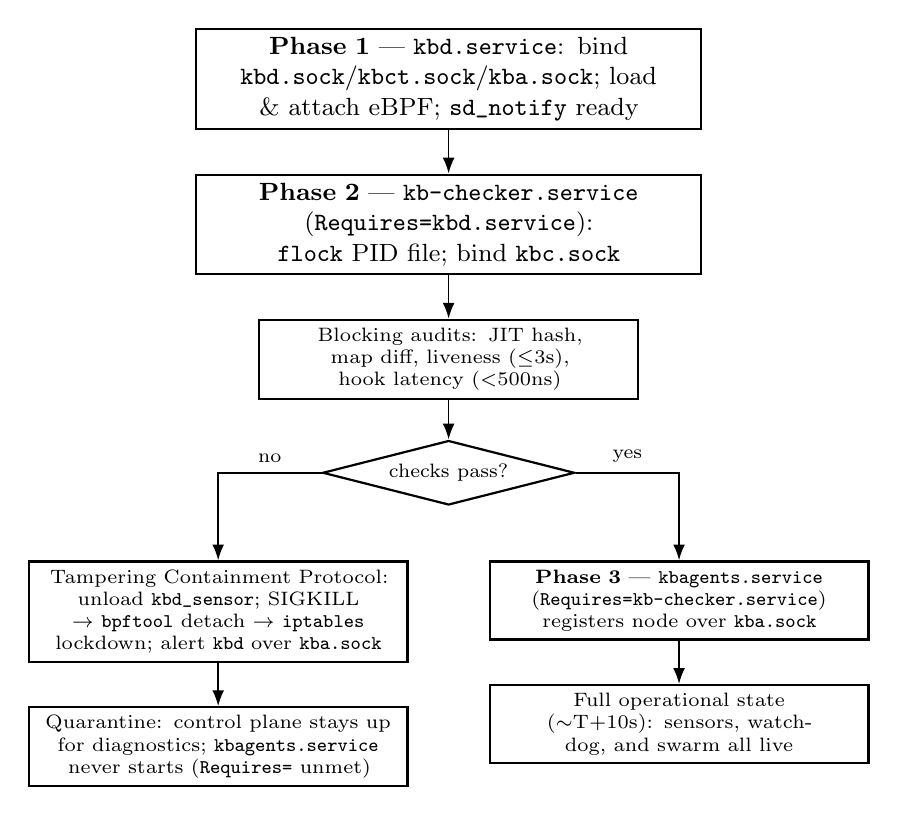
\begin{tikzpicture}[
  stg/.style={draw, thick, minimum height=0.9cm, text width=6.2cm,
    align=center, font=\small, inner sep=3pt},
  small/.style={draw, thick, minimum height=0.8cm, text width=4.6cm,
    align=center, font=\scriptsize, inner sep=3pt},
  dec/.style={draw, thick, diamond, aspect=3, align=center, font=\scriptsize, inner sep=1pt},
  >=Latex, line width=0.6pt, color=black, node distance=0.55cm
]
\node[stg] (s1) {\textbf{Phase 1} --- \texttt{kbd.service}: bind \texttt{kbd.sock}/\texttt{kbct.sock}/\texttt{kba.sock}; load \& attach eBPF; \texttt{sd\_notify} ready};
\node[stg, below=of s1] (s2) {\textbf{Phase 2} --- \texttt{kb-checker.service} (\texttt{Requires=kbd.service}): \texttt{flock} PID file; bind \texttt{kbc.sock}};
\node[small, below=of s2] (s3) {Blocking audits: JIT hash, map diff, liveness ($\leq$3s), hook latency ($<$500ns)};
\node[dec, below=0.5cm of s3, minimum width=3.2cm] (d1) {checks pass?};

\node[small, below left=0.9cm and -0.3cm of d1] (fail) {Tampering Containment Protocol: unload \texttt{kbd\_sensor}; SIGKILL $\to$ \texttt{bpftool} detach $\to$ \texttt{iptables} lockdown; alert \texttt{kbd} over \texttt{kba.sock}};
\node[stg, text width=4.6cm, below=of fail, font=\scriptsize] (quarantine) {Quarantine: control plane stays up for diagnostics; \texttt{kbagents.service} never starts (\texttt{Requires=} unmet)};

\node[small, below right=0.9cm and -0.3cm of d1] (pass) {\textbf{Phase 3} --- \texttt{kbagents.service} (\texttt{Requires=kb-checker.service}) registers node over \texttt{kba.sock}};
\node[stg, text width=4.6cm, below=of pass, font=\scriptsize] (full) {Full operational state ($\sim$T+10s): sensors, watchdog, and swarm all live};

\draw[->] (s1) -- (s2);
\draw[->] (s2) -- (s3);
\draw[->] (s3) -- (d1);
\draw[->] (d1) -| node[pos=0.25, above, font=\scriptsize] {no} (fail);
\draw[->] (d1) -| node[pos=0.25, above, font=\scriptsize] {yes} (pass);
\draw[->] (fail) -- (quarantine);
\draw[->] (pass) -- (full);
\end{tikzpicture}
\caption{Boot sequence and daemon-lifecycle gating (\S\ref{sec:boot}).
Every arrow crossing a phase boundary corresponds to a real
\texttt{systemd} \texttt{After=}/\texttt{Requires=} dependency, not
application-level polling --- a failed or absent \texttt{kb-checker}
structurally prevents \texttt{kbagents.service} from starting, the
same way \texttt{systemd} would block any unit depending on a failed
one.}
\label{fig:boot}
\end{figure*}

\subsection{Fail-Safe Paths}

Three failure modes are handled explicitly, not left to silent
retries. An \textbf{eBPF hook loading failure} (no LSM support, or
\texttt{kbd\_sensor} fails to attach) means \texttt{kbd} never sends
its readiness signal, so \texttt{kb-checker} --- gated on that signal
--- never starts, and neither does the swarm. A \textbf{UDS socket
loss} (e.g.\ \texttt{kbd} restarting mid-run, briefly deleting
\texttt{kba.sock}) is tolerated for up to 15s of retries before
\texttt{kb-checker} treats it as a containment-worthy event and forces
an emergency bytecode reload. \textbf{Graceful termination}
(\texttt{systemctl stop kb-checker}) is a real code path, not just
process death: \texttt{kb-checker} catches \texttt{SIGTERM}, stops its
audit loops, closes its gRPC server, and removes both
\texttt{kbc.sock} and its own PID-lock file before exiting, so a
deliberate stop never leaves stale state for the next start to trip
over.

\subsection{Chronological Timeline}
\label{sec:boot-timeline}

\Cref{tab:boot-timeline} gives the same three phases as a single
concrete timeline, with the approximate wall-clock offsets from
power-on the boot-sequence specification records for a representative
boot --- the phase boundaries in \Cref{fig:boot} are the
\texttt{After=}/\texttt{Requires=} dependencies; this is how long each
side of them actually takes in practice.

\begin{table}[h]
\centering
\scriptsize
\renewcommand{\arraystretch}{0.95}
\caption{Chronological boot sequence, power-on to full operational state.}
\label{tab:boot-timeline}
\begin{tabular}{@{}p{1.1cm}p{6.2cm}@{}}
\toprule
Offset & Event \\
\midrule
T+0.00s & Power-on: UEFI/GRUB verify and measure the boot chain; initramfs and root filesystem mount; \texttt{systemd} (PID 1) takes control \\
T+4.50s & \textbf{Phase 1}: \texttt{kbd.service} binds sockets, loads eBPF, sends \texttt{sd\_notify} ready \\
T+6.00s & \textbf{Phase 2}: \texttt{kb-checker.service} spawns (\texttt{After=kbd}), locks its PID file, runs blocking audits \\
T+7.50s & Decision: pass $\to$ loops; fail $\to$ Containment Protocol \\
T+8.50s & \textbf{Phase 3}: \texttt{kbagents} starts if Phase 2 passed (else blocked) and registers over \texttt{kba.sock} \\
T+10.00s & Full operational state: all subsystems live \\
\bottomrule
\end{tabular}
\end{table}
\FloatBarrier

\section{kb-op: Operator Interfaces}
\label{sec:op}

\texttt{kb-op} provides four operator-facing surfaces over KB's gRPC
and HTTP APIs.

\subsection{kbctl}

\texttt{kbctl} is a Go CLI dialing \texttt{kbd}'s gRPC service directly
over its Unix domain socket. It supports process isolation and restore
(\texttt{process isolate}, with an explicit
\texttt{CGROUP|SECCOMP|NAMESPACE|TERMINATE} level flag), zone
classification overrides, audit-chain verification and JSON export
(\texttt{audit verify}, \texttt{audit export}), policy hot-reload
(\texttt{policy reload}), system statistics, and CWP workload key
generation and signing (\texttt{workload keygen}, \texttt{workload
sign}, \S\ref{sec:cwp-sign}). An earlier revision of this paper's audit
reported \texttt{audit verify} as calling \texttt{os.Exit(1)} directly
on a detected chain break, bypassing its own deferred cleanup; current
source returns the failure through Cobra's normal \texttt{RunE} error
path instead, letting every \texttt{defer} run --- this claim did not
hold up against current code and is corrected here rather than carried
forward.

\subsection{kb-tui}

\texttt{kb-tui} is a Rust/ratatui terminal console. An earlier revision
of this paper described it as reachable over a custom, hand-rolled Go
SSH server hosted in-process by \texttt{kbd} (\texttt{internal/ssh/}),
with a security migration to real OpenSSH recorded only as a
considered, not-yet-implemented future decision. That migration is, in
fact, already complete: \texttt{internal/ssh/} has been deleted from
\texttt{kb-control-plane} in full, and port 2222 is now served by a
second, independent instance of the system's own \texttt{sshd}
(\texttt{sshd@kb-operator.service}), configured with
\texttt{ForceCommand} to exec \texttt{kb-tui} directly after real
OpenSSH authentication --- \texttt{kbd} retains no host keys,
\texttt{authorized\_keys} parsing, or PTY code of its own. This
resolves both defects an earlier revision of this audit attributed to
the retired custom server (no login-attempt throttling; a dev-mode host
key path that could silently relocate key material) by removing the
component they applied to, not by patching it --- real \texttt{sshd}'s
own decades-old hardening (rate limiting via PAM/\texttt{fail2ban}
conventions, fixed host-key handling) now governs this listener
entirely. \texttt{kbctl}'s hidden \texttt{ssh} subcommand is the
audit-callback glue this design still needs: it is invoked by the
\texttt{ForceCommand} wrapper script (not run interactively) to record
session metadata (principal, remote address, identity) against the
audit log.

\subsection{kb-dashboard}

\texttt{kb-dashboard} is a TypeScript web frontend against \texttt{kbd}'s
HTTP API. An earlier revision of this paper reported its isolate/restore
controls as the client side of an unauthenticated, wildcard-CORS API
with a hardcoded \texttt{localhost:8080} host. Current source does not
match that description: the API base resolves from
\texttt{window.location.hostname} (overridable via
\texttt{VITE\_KB\_API\_BASE} for a non-local deployment) rather than a
hardcoded host, and isolate/restore requests carry a bearer token from
\texttt{VITE\_KB\_API\_TOKEN} matching the server's
\texttt{KB\_HTTP\_API\_TOKEN} (\S\ref{sec:cp}) --- the dashboard's own
source comments this fix as tied directly to that server-side change.
This is corrected here rather than repeated.

\subsection{kb-mcp}

\texttt{kb-mcp} exposes KB's telemetry and query surface as a Model
Context Protocol server, intended to let LLM-based tooling query
process state and zone classifications through the same gRPC API
\texttt{kbctl} and \texttt{kb-tui} use. This subsystem was not included
in the source-level audit reported in \S\ref{sec:audit}.

\section{Security Audit}
\label{sec:audit}

Independent of any single subsystem's feature work, we conducted a
source-level audit across \texttt{kb-core}, \texttt{kb-control-plane},
\texttt{kb-aads}, and \texttt{kb-op} (\texttt{kb-checker} was included
in scope but no defects were found within the time available, and
\texttt{kb-mcp} specifically was not covered). An earlier revision of
this audit reported fifteen open defects, five of them summarized in a
severity table; re-verifying every one of those claims directly against
current source for this revision --- rather than continuing to carry
them forward --- found that the great majority no longer hold: they
were already fixed in team history that simply predates when this
paper's audit text was originally drafted, and were never re-checked
against current code before being repeated. This is, itself, worth
stating plainly as a methodological finding: a security audit's claims
decay the moment the underlying code moves, and re-verifying against
current source before every revision is not optional. Specifically
confirmed already fixed, and corrected in this revision rather than
left stale: the unauthenticated wildcard-CORS HTTP API (bearer-token
auth plus an origin allowlist now gate it, \S\ref{sec:cp}), the
telemetry-update containment-reset bug (\texttt{UpsertProcessState}
explicitly preserves containment across updates, \S\ref{sec:cp}), the
LSM level-3+ fail-open ordering (\S\ref{sec:core}), the custom SSH
server's missing throttling and dev-mode host-key fallback (the server
itself was deleted and replaced by real \texttt{sshd}, \S\ref{sec:op}),
the dashboard's hardcoded API host (\S\ref{sec:op}), absent input
validation/rate limiting on containment RPCs (existence checks and
per-agent throttling are tested, \S\ref{sec:cp}), \texttt{kbctl}'s
claimed \texttt{os.Exit(1)} cleanup bypass (not present in current
source, \S\ref{sec:op}), and Jury's three previously-reported consensus
defects (\S\ref{sec:jje}). One claim was re-verified and confirmed
genuinely still open: the audit-chain verifier's missing
\texttt{rows.Err()} check (\S\ref{sec:audit-log}), which is fixed in
this revision with a dedicated regression test. At the time of writing
we are not aware of any other confirmed-open defect in the four audited
subsystems beyond what is discussed alongside each subsystem above;
this reflects the scope and time available for this revision's
re-verification pass, not a claim of exhaustive proof.

\begin{table}[htbp]
\centering
\footnotesize
\caption{Status of every defect this paper has, at some revision,
reported as open. ``Predates audit'' means current source already
fixed it before this paper's audit text was first drafted.}
\label{tab:bugs}
\begin{tabular}{@{}p{1.5cm}p{1.9cm}p{3.9cm}@{}}
\toprule
ID & Status & Summary \\
\midrule
BUG-001 & Fixed (predates audit) & HTTP API had no auth, wildcard CORS (\S\ref{sec:cp}) \\
BUG-002 & Fixed (predates audit) & Telemetry reset active containment to NONE (\S\ref{sec:cp}) \\
BUG-004 & Fixed (predates audit) & LSM hook could fail open on path-resolution failure (\S\ref{sec:core}) \\
BUG-005 & \textbf{Fixed this revision} & Audit verifier never checked \texttt{rows.Err()} (\S\ref{sec:audit-log}) \\
BUG-006 & Moot (component removed) & Custom SSH throttling gap; server since deleted (\S\ref{sec:op}) \\
\bottomrule
\end{tabular}
\end{table}

\section{Current Project Status}
\label{sec:status}

\Cref{tab:status} summarizes what is complete, partial, or outstanding
across all five subsystems this paper covers at the time of writing.
NOMAD (\S\ref{sec:nomad}), developed in a separate repository, is
excluded from this table.

\begin{table}[htbp]
\centering
\footnotesize
\caption{Per-subsystem implementation status.}
\label{tab:status}
\begin{tabular}{@{}p{1.5cm}p{5.6cm}@{}}
\toprule
Subsystem & Status \\
\midrule
kb-core (\S\ref{sec:core}) & Complete for the enforcement primitives
documented here, each independently live-verified, including a new
userspace-only network-flow wire message for exfiltration detection.
Both LSM fail-open-ordering and PID-keyed-map-exhaustion claims from an
earlier audit revision are confirmed already fixed on re-verification. \\
kb-control-plane (\S\ref{sec:cp}) & Complete for storage, scoring
ingestion, gRPC/HTTP API, audit-chain logging, policy hot-reload,
signed CWP workload policy, severity escalation, and exfiltration/
beaconing detection. 128 tests passing. HTTP API auth/CORS and the
containment-reset bug were already fixed in prior history; the
audit-chain \texttt{rows.Err()} gap is fixed in this revision. \\
kb-aads (\S\ref{sec:aads}) & Actor scaffolding functional. Containment
and Jury roles carry trained, live-verified RL policies. Patroller and
Healer carry real rule-based logic. Containment militia, signal
relays, and \texttt{SwarmRegistry}-backed JJE courthouse oversight are
newly implemented. Hunter remains a non-functional stub, by design a
separate, larger undertaking. 68 tests passing. \\
kb-checker (\S\ref{sec:checker}) & Complete for its stated scope
(stateless integrity auditing, boot-sequence gating, fallback
containment), now included in CPM's protected floor. No defects found
in this audit within the time available. \\
kb-op (\S\ref{sec:op}) & \texttt{kbctl}, \texttt{kb-tui}, and
\texttt{kb-dashboard} functional against the current gRPC/HTTP
surface; \texttt{kbctl} gained CWP workload key generation/signing.
\texttt{kb-tui}'s SSH transport migrated to a real, independent
\texttt{sshd} instance, superseding and removing the custom Go SSH
server this paper's earlier audit revision evaluated. \texttt{kb-mcp}
functional per its own scope but not included in this audit's
coverage. \\
\bottomrule
\end{tabular}
\end{table}

\section{Limitations and Future Work}

Several gaps are explicitly acknowledged rather than papered over.
KB's own attack-lab data pipeline remains unbuilt, so Containment and
Jury's shared training data (\S\ref{sec:rl}, \S\ref{sec:jury-rl}) is a
public-dataset stand-in with no coverage for the
\texttt{memory\_exploit} scenario, and no mapping yet exists from
\texttt{kb-core}'s real eBPF event-type vocabulary to the category
codes that policy was trained on. Hunter requires both a fine-tuned
agentic LLM tool-call loop and its own training data, neither of which
exists yet. Healer's decision remains rule-based, not learned, because
the restore-outcome ground truth its reward would require does not
exist in this codebase. The JJE courthouse's severity classifier
(\Cref{eq:courthouse}) only ever reaches \texttt{restart}
automatically; \texttt{revoke} and \texttt{terminate} require signal
producers (peer-baseline drift detection, authorization-boundary
violation detection) that have not been built, and its own
quorum-gating design is not implemented for the reason given in
\S\ref{sec:courthouse}. \texttt{kb-mcp} was not covered by this audit
cycle. NOMAD (\S\ref{sec:nomad}) is out of this paper's own scope,
tracked and developed independently; its parallel repository's own
documentation flags PCR-bank selection and re-sealing ownership, the
SBC/STM32/ESP32 internal protocol, and the FMS wire protocol as
unresolved design questions there, separate from anything this paper
is responsible for. On the security-audit front specifically: this revision's
re-verification pass found that most previously-reported open findings
were already fixed in code that predates when this paper's audit text
was first drafted, which is itself a limitation worth stating plainly
--- an audit's claims are only as current as the last time they were
checked against real source, and this paper's own earlier revision went
uncorrected for some time. The one defect re-verification confirmed
genuinely open (\S\ref{sec:audit-log}'s \texttt{rows.Err()} gap) is
fixed in this revision. We are not aware of a remaining critical,
unauthenticated enforcement surface in current source, but this
reflects the scope and time available for this pass, not a claim of
exhaustive security review; a fresh, independent audit before any
production deployment remains warranted regardless.

\section{Conclusion}

We documented Kernel Borderlands subsystem by subsystem: kernel-verified
enforcement primitives and authorization gates in \texttt{kb-core}; a
two-tier storage engine, hash-chained audit log, hot-reloadable policy
engine, signed workload policy, and statistical exfiltration detection
in \texttt{kb-control-plane}; an actor-based swarm in \texttt{kb-aads}
now carrying two trained and live-verified reinforcement-learning
decision roles (Containment and Jury), real rule-based Patroller and
Healer logic, a mechanically-sequenced containment militia, dedicated
signal-relay actors, and a registry-backed courthouse oversight
mechanism for the swarm itself; a stateless boot-gating watchdog in
\texttt{kb-checker}, now extended with a briefly-noted, separately and
actively developed hardware trust module, NOMAD, addressing the one
failure mode no same-host software component can structurally cover
(total kernel compromise), though not itself a subject this paper
documents in depth; and four operator interfaces in \texttt{kb-op}.
We gave a single, consolidated mathematical
formulation covering every learned and statistically-driven decision
procedure in the system, and subjected the four implemented,
non-hardware subsystems to the same source-level security scrutiny
this paper's audit reports throughout. Re-verifying that audit's own
prior claims against current source for this revision --- rather than
repeating them --- found the great majority already resolved, fixed
one genuine remaining defect (an audit-chain integrity check silently
masking a class of I/O error) with a dedicated regression test, and
corrected several since-superseded claims (a migrated SSH transport, an
already-authenticated HTTP API) that an earlier revision had continued
to describe as open or as future work. A fresh, independent audit
before any production deployment remains warranted regardless of this
finding.

\bibliographystyle{unsrtnat}
\bibliography{references}

\end{document}
